Etant donné que ce plugin doit pouvoir s'intégrer aux différents sites SPIP, il doit pouvoir utiliser les systèmes déjà mis en place. Les nouvelles tables ajoutées pour le fonctionnement de ce plugin se rattachent donc à des tables déjà existantes du système SPIP.\\
\newline
On retrouve les différentes tables suivantes :

\vspace{0.5cm}

\begin{figure}[h]
    \centering
    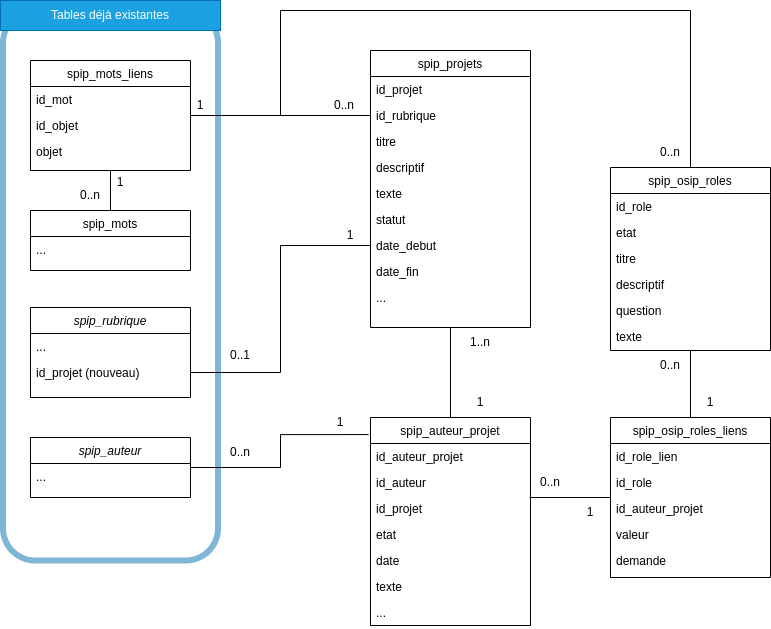
\includegraphics[trim=0 0 0 0, clip, width=1\textwidth]{images/table_plugin_projet.drawio.png}
    \caption{Tables du plugins "OSI\_Projets"}
    \label{Tables du plugin osiprojets}
\end{figure}
\newpage
On peut voir que ce plugin fonctionne grâce à quatre nouvelles tables : 
\begin{itemize}
    \item \texttt{spip\_projets} : Table qui représente les "projets" (groupe d'auteurs). L'idée est ici de se rattacher à un type de page déjà présent sur le front (ici une rubrique) pour pouvoir profiter des fonctionnalités déjà présentes sur cette dernière en ajoutant celles nécessaires pour le fonctionnement du plugin.
    \item \texttt{spip\_auteur\_projet} : Table qui représente le lien entre un auteur et un projet. L'état permet de représenter les différents niveaux de droits sur le projet. Cette table représente aussi les demandes pour rejoindre un projet.
    \item \texttt{spip\_osip\_roles} : Table qui représente des rôles que peuvent obtenir les membres d'un projet.
    \item \texttt{spip\_osip\_roles\_liens} : Table qui représente le lien entre un rôle et un membre d'un projet. C'est aussi la table qui représente les demandes pour obtenir un rôle ou non. 
\end{itemize}
En regardant les tables de la figure \ref{Tables du plugin osiprojets}, on peut voir qu'un projet peut accueillir autant d'auteurs que possible, mais avec un minimum d'un auteur (le créateur du projet). \\
\newline
Comme il a été dit précédemment, le niveau de droit d'un utilisateur par rapport à un projet est réalisé grâce à la colonne \texttt{etat} d'un élément de la table \textit{spip\_auteur\_projet}. En effet, on retrouve les niveaux d'état suivants : 
\begin{itemize}
    \item 3 - Créateur du projet
    \item 2 - Administrateur du projet
    \item 1 - Membre du projet
    \item 0 - Utilisateur ayant fait une demande pour rejoindre le projet
    \item -1 - Utilisateur ayant fait une demande pour rejoindre le projet qui a été refusée
    \item -2 - Utilisateur qui a été banni du projet
\end{itemize}
